\documentclass[11pt]{article}
\usepackage{amsthm, amsmath, amssymb, amsfonts, url, booktabs, tikz, setspace, fancyhdr, bm}
\usepackage{tikz}
\usepackage{xcolor}

\begin{document}

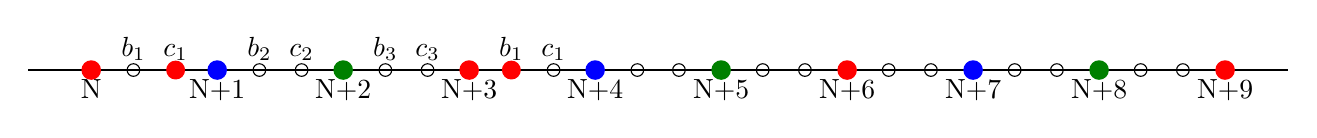
\begin{tikzpicture}[scale=0.8]
    % Draw the x-axis
    \draw[-] (-10,0) -- (10,0);
    
    % Define the colors
    \definecolor{red}{RGB}{255,0,0}
    \definecolor{blue}{RGB}{0,0,255}
    \definecolor{green}{RGB}{0,128,0}
    
    % Draw the colored dots
    \foreach \x/\color/\label in {-9/red/N, -7/blue/N+1, -5/green/N+2, -3/red/N+3, -1/blue/N+4, 1/green/N+5, 3/red/N+6, 5/blue/N+7, 7/green/N+8, 9/red/N+9} {
        \node[circle, fill=\color, inner sep=2.5pt] at (\x,0) {};
        \node[below] at (\x,0) {\label};
       
        

        
    }
     \draw (-7.66,0) circle (0.1) node [above]{$c_{1}$};
     \fill[red](-7.66,0) circle (0.15);
     \draw (-5.66,0) circle (0.1)node [above]{$c_{2}$};
     \draw (-3.66,0) circle (0.1)node [above]{$c_{3}$};
     \draw (-1.66,0) circle (0.1)node [above]{$c_{1}$};
     \draw (0.33,0) circle (0.1);
     \draw (2.33,0) circle (0.1);
     \draw (4.33,0) circle (0.1);
     \draw (6.33,0) circle (0.1);
     \draw (8.33,0) circle (0.1);

     
     \draw (-8.33,0) circle (0.1)node [above]{$b_{1}$};
     
     \draw (-6.33,0) circle (0.1)node [above]{$b_{2}$};
     \draw (-4.33,0) circle (0.1)node [above]{$b_{3}$};
     \draw (-2.33,0) circle (0.1)node [above]{$b_{1}$};
\fill[red](-2.33,0) circle (0.15);
     
     \draw (-0.33,0) circle (0.1);
     \draw (1.66,0) circle (0.1);
     \draw (3.66,0) circle (0.1);
     \draw (5.66,0) circle (0.1);
     \draw (7.66,0) circle (0.1);
     



    
\end{tikzpicture}

\end{document}